\chapter{Stereo video watermarking}
\markright{Stereo video watermarking}
\label{wat}
\phantomsection
%\addcontentsline{toc}{chapter}{Stereoscopic Video}

\section{Watermaking}

Digital watermarking consists in imperceptiby and persistently associating some extra information with some original content. \\
The basic watermarking workflow is presented in Figure \ref{fig:workflow}.\\
\begin{figure}[h!]
\centering
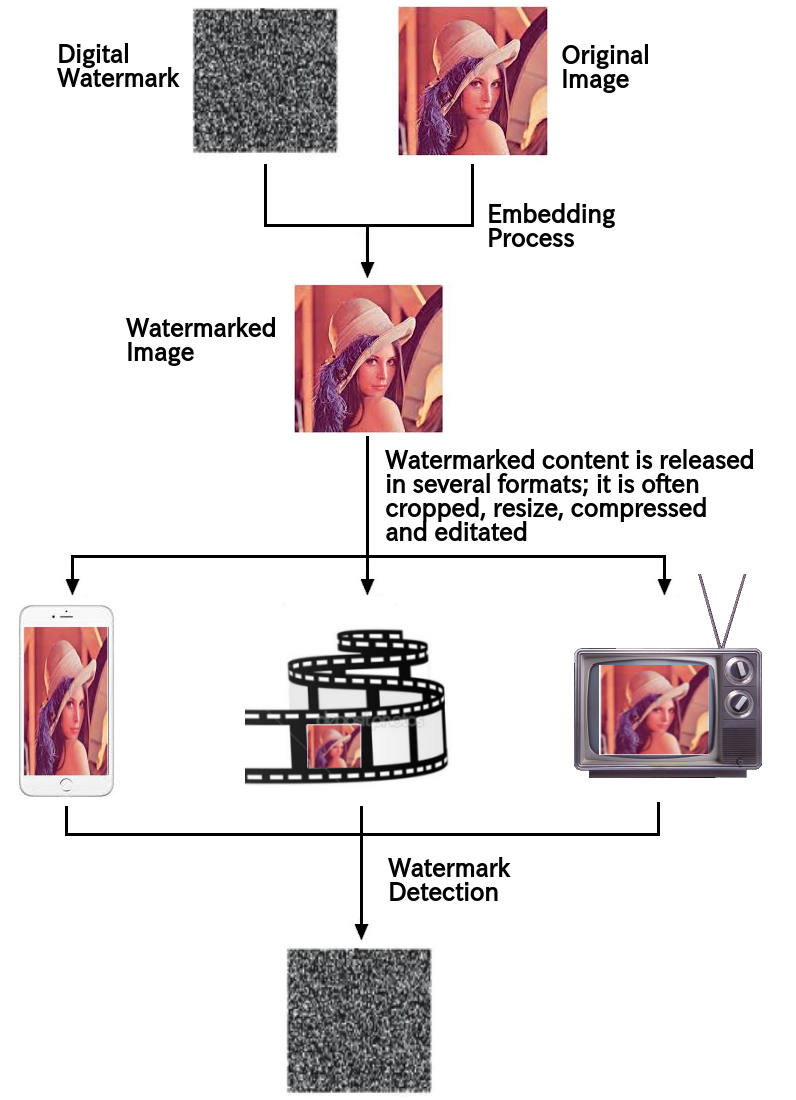
\includegraphics[width=0.3\textwidth]{./img/wat_workflow.png}
\caption{\small{Watermarking workflow}}
\label{fig:workflow}
\end{figure}
\newpage
\subsection{Properties}
Three parameters are required to evaluate watermarking technique performances:
\begin{itemize}
\item[-] transparency, that is the misure of how much the watermark affects the quality of the host data;
\item[-] robustness, i.e.,the capability of the hidden data to survive host signal manipulation including compression, signal processing, geometric manipulations;
\item[-] data payload, that is the amount of data of information bits that it is able to convey.
\end{itemize}
\begin{figure}[h!]
\centering
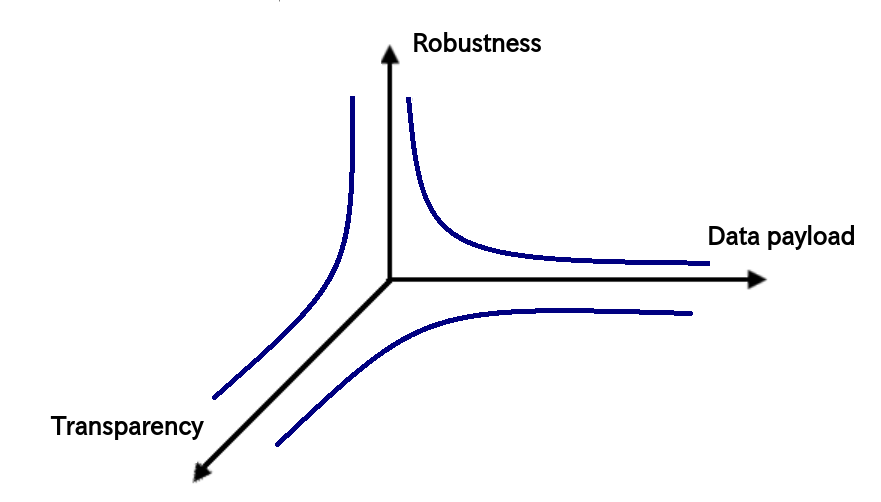
\includegraphics[width=0.4\textwidth]{./img/properties.png}
\caption{\small{Watermark properties trade-off}}
\label{fig:properties}
\end{figure}

To evaluate the quality of the watermarking technique in terms of transparency the measures in \cite{QMETRICS} have been used.\\
In Chaminda et al.'s study a Reduced-Reference
(RR) quality metric for color plus depth 3D video compression and transmission is proposed, using the extracted edge information of color plus depth map 3D video.\\ 
The work is motivated by the fact that the edges/contours of the depth map can represent different depth levels and this can be considered for measuring structural degradations. Since depth map boundaries are also coincident with the corresponding color image object boundaries, edge information of the color image and of the depth map is compared to obtain a quality index (structural degradation) for the corresponding color image sequence.\\
In order to quantify structural comparison, luminance comparison and contrast comparison parameters for the depth map and corresponding watermarked views, a modified version of the
commonly used SSIM metric is adopted:
\begin{equation}
Q_{Depth}(x,y) = [l(x,y)]^{\alpha} \cdot [c(x,y)]^{\beta} \cdot [\mathnormal{S}_{Depth}(x',y')]^{\gamma}
\end{equation}
where $l(x,y)$ and $c(x,y)$ are luminance and contrast comparisons performed on original depth maps and the ones computed after watermarking,
respectively, and $\mathnormal{S}_{Depth}(x',y')$  is the structural comparison between the gradient/edge maps of original and post-watermarking computed depth map images.\\
Then the overall depth map quality is calculated as
\begin{equation}
MQ_{Depth}(X,Y) = \frac{1}{M} \sum_{j=1}^{M}Q_{Depth}(x_{j},y_{j}).
\end{equation}
The SSIM-based quality index for the color image can be described as follows:
\begin{equation}
Q_{View}(x,y) = [l(x,y)]^{\alpha} \cdot [c(x,y)]^{\beta} \cdot [\mathnormal{S}_{View}(x',y')]^{\gamma}
\end{equation}
where $l(x,y)$ and $c(x,y)$ are luminance and contrast comparisons performed on original and watermarked views, respectively, and $\mathnormal{S}_{View}(x',y')$  is the structural comparison between the gradient/edge maps of the gradient maps of the corresponding original depth map and the watermarked views.\\
Hence, the overall color image quality is calculated as
\begin{equation}
MQ_{View}(X,Y) = \frac{1}{M} \sum_{j=1}^{M}Q_{View}(x_{j},y_{j}).
\end{equation}
As in \cite{QMETRICS}, the Sobel
operator has been selected to obtain edge information (i.e., the binary edge mask) due to its simplicity and efficiency.\\

Since in stereoscopic video context it is rather common practice to generate intermediate virtual views to adjust depth perception and since such view synthesis introduces non-rigid local geometric distortion that are not properly tackled by state-of-the art resynchronization mechanisms, stereo video watermarking strategies have to achieve robustness to synthetic view synthesis.\\
In this thesis a disparity-coherent method has been implemented since this class of watermarking technique are expected to exhibit superior robustness against view synthesis.\\

Finally, a watermarking technique can be:
\begin{itemize}
\item[-] non-blind/blind, if at the decoder side the original content is available or not, respectively;
\item[-] private, if only authorized users
can recover it, otherwise it's public;
\item[-] detectable, if it is only possible to decide whether a given watermark is embedded in the content, privateness is automatically achieved; otherwise the watermark readable watermark the bits hidden in the content can be read without
knowing them in advance


\end{itemize}




\subsection{Embedding techniques}
The most straightforward ways to add a watermark in a given content have been proved to be Spread Spectrum (SS) approach and Side Information (SI).\\
\begin{figure}[h!]
\centering
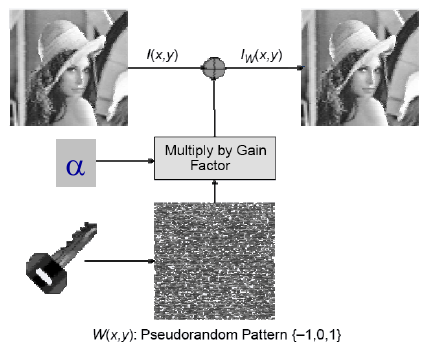
\includegraphics[width=0.4\textwidth]{./img/ss.png}
\caption{\small{Spread spectrum technique}}
\label{fig:ss}
\end{figure}
As in spread spectrum communications, the former approach considers the original
content as a signal and the watermark as a noise that is spread over very many frequency bins so that the energy in any one bin is very small and certainly undetectable.\\
The latter takes advantage of the fact that the original content is known at the
embedder side (but unknown at the detector): this way the watermark can be modulated  according to the original and the quantity of
inserted data can be maximed.\\

Sometimes hybrid watermarking methods combining spread spectrum and side information concepts can be applied; they try to benefit from both the robustness and transparency of the spread
spectrum methods and the increased data payload of the side information methods.
\begin{figure}[h!]
\centering
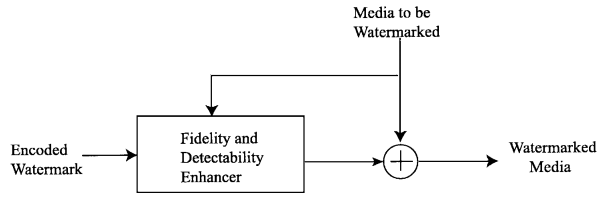
\includegraphics[width=0.5\textwidth]{./img/si.png}
\caption{\small{Side information technique scheme}}
\label{fig:si}
\end{figure}


\subsection{Embedding domains}
Host features modified during embedding can
belong to 
\begin{itemize}
\item[-] spatial domain: the watermark is embedded by directly modifying the pixel values;
\begin{figure}[h!]
\centering
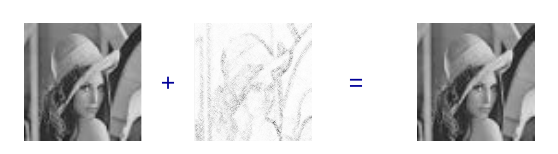
\includegraphics[width=0.4\textwidth]{./img/domain1.png}
\caption{\small{Spatial domain watermark insertion}}
\label{fig:dom1}
\end{figure}
\item[-] frequency domain: the image is transformed through a mathematical transformation, some coefficients are modified and finally the inverse transform is carried out;
\begin{figure}[h!]
\centering
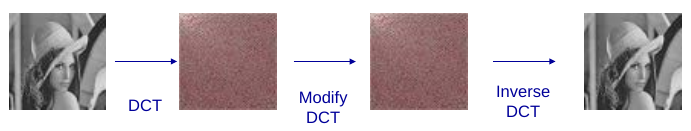
\includegraphics[width=0.4\textwidth]{./img/domain2.png}
\caption{\small{Frequency domain watermark insertion}}
\label{fig:dom2}
\end{figure}
\item[-] hybrid techniques: a block wise transform is applied, the image is divided
into blocks and for each block a mathematical transformation is computed, some coefficients are modified and the inverse transform is done.
\begin{figure}[h!]
\centering
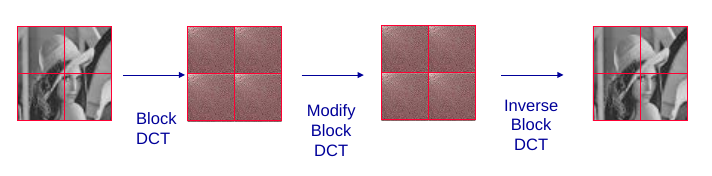
\includegraphics[width=0.4\textwidth]{./img/domain3.png}
\caption{\small{Hybrid technique}}
\label{fig:dom3}
\end{figure}
\end{itemize}

In stereoscopic video context the studies can also be structured in two other categories:
\begin{itemize}
\item[-] view-based methods;
\item[-] disparity-based methods
\end{itemize}
according to the reference image in which the mark is actually inserted.\\
In Figure \ref{stereo_method} the workflows of both methods are presented.
\begin{figure}[h!]
\centering
\begin{subfigure}[]{0.4\textwidth}
\centering
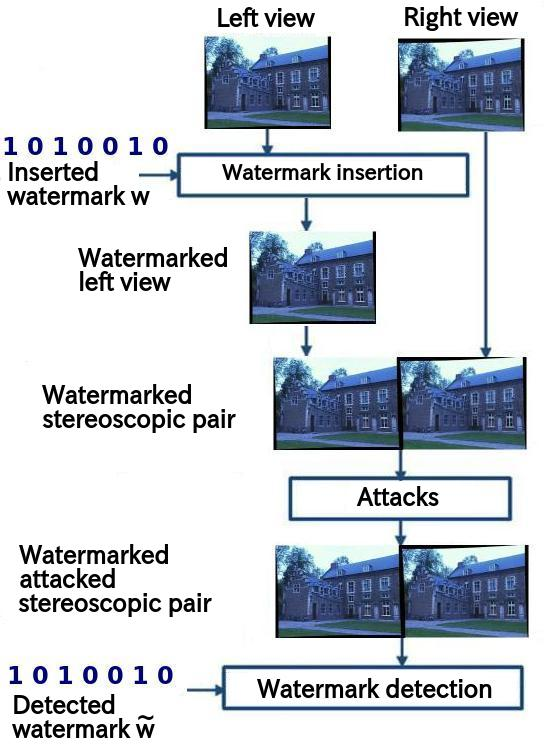
\includegraphics[width=0.8\textwidth]{./img/views_domain.jpeg}
\caption{\small{View-based watermarking workflow}}
\label{fig:view}
\end{subfigure}% 
~ %add desired spacing between images, e. g. ~, \quad, \qquad,  etc.$  $
  %(or a blank line to force the subfigure onto a new line)
\begin{subfigure}[]{0.4\textwidth}
\centering
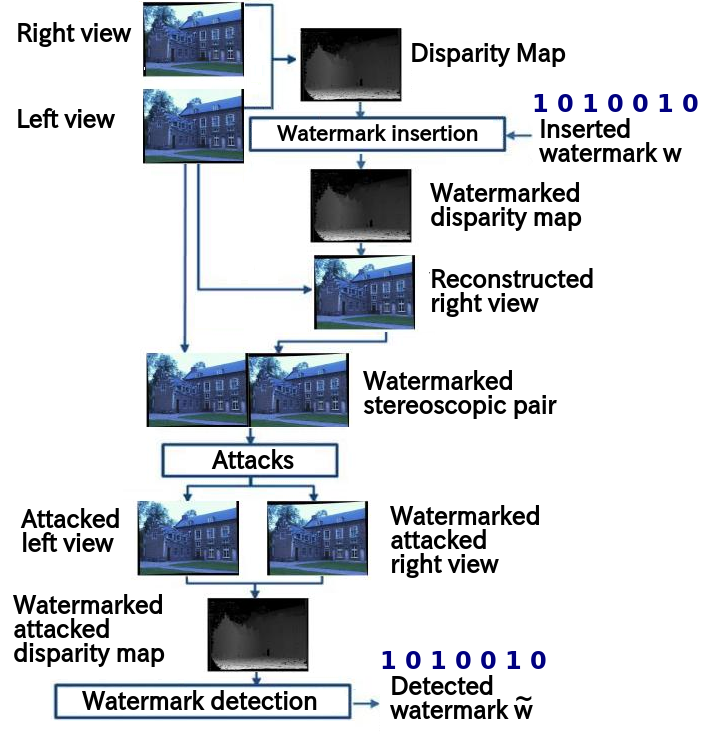
\includegraphics[width=1.05\textwidth]{./img/disparity_domain.png}
\caption{\small{Disparity-based watermarking workflow}}
\label{fig:disp}
\end{subfigure}
\caption{\small{Stereoscopic video watermarking workflow}\label{stereo_method}}
\end{figure}







\newpage
In this thesis ....
due algoritmi di marchiatura presentati; il primo spaziale ss con rumore gaussiano etc.. 
il secondo ss nella frequenza additivo moltiplicativo...


data payload è ...
la trasparenza è stata valutata con ...
la robustezza è stata provata per view synthesis e compressione



